\begin{figure}[t]
  \centering
  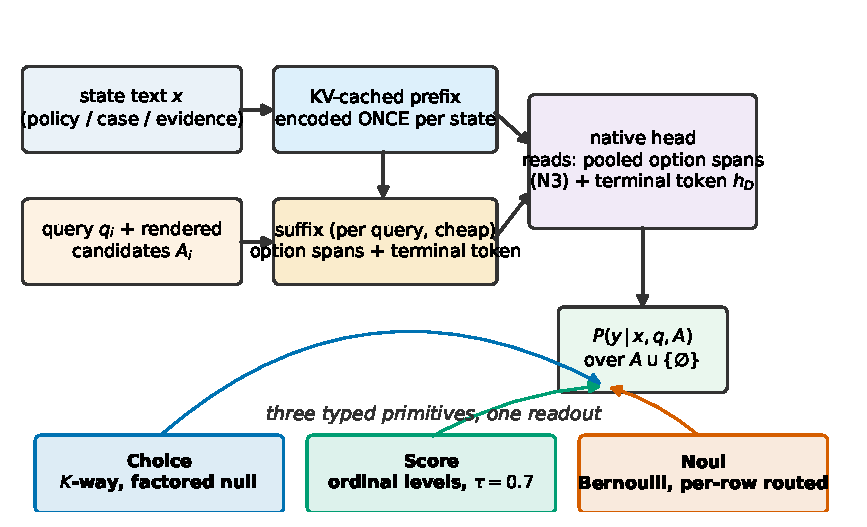
\includegraphics[width=\linewidth]{figures/fig_architecture.pdf}
  \caption{Schematic of the decision pass: KV-cached state prefix, per-query suffix, native head reading pooled option spans + terminal token, three typed primitives (Choice / Score / Noul) on one readout.}
  \label{fig:architecture}
\end{figure}

\begin{figure}[t]
  \centering
  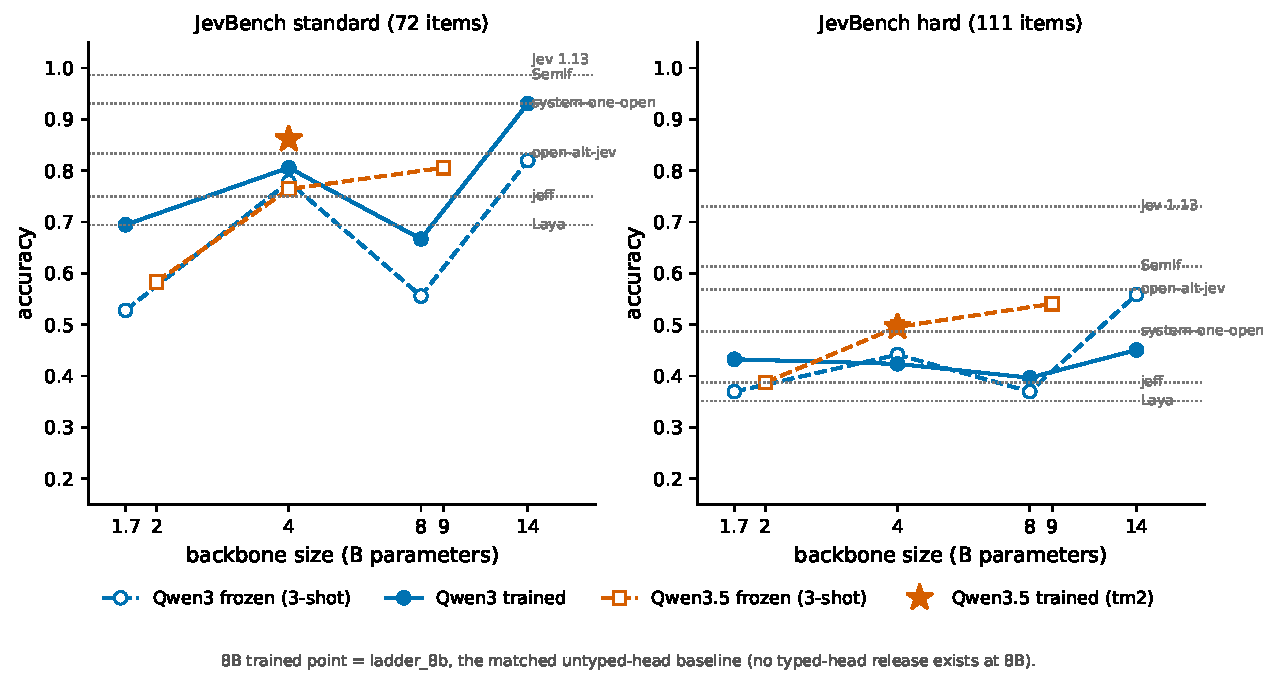
\includegraphics[width=\linewidth]{figures/fig_ladder.pdf}
  \caption{JevBench standard and hard accuracy vs backbone size for Qwen3 (1.7/4/8/14B) and Qwen3.5 (2/4/9B); frozen-with-3-shots dashed, trained solid; open-field references as horizontal markers.}
  \label{fig:ladder}
\end{figure}

\begin{figure}[t]
  \centering
  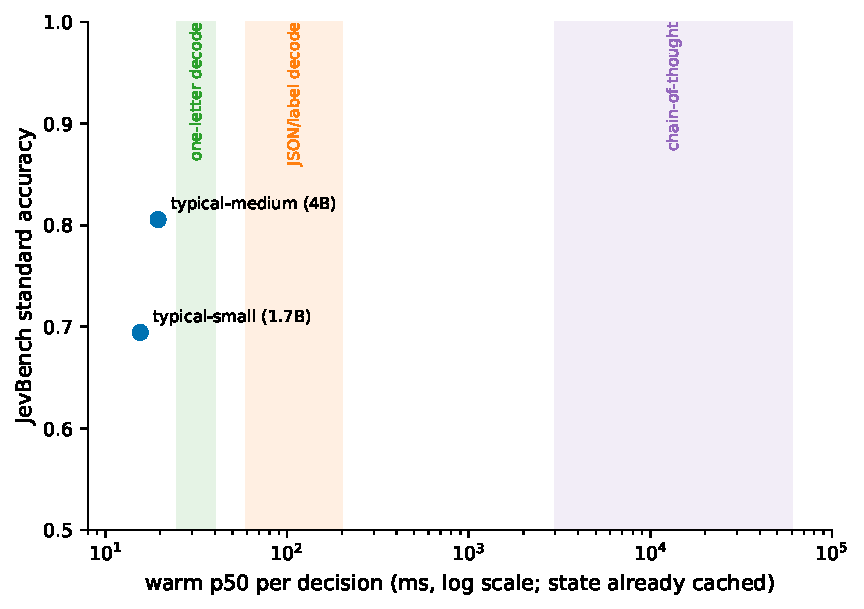
\includegraphics[width=\linewidth]{figures/fig_latency_quality.pdf}
  \caption{JevBench standard accuracy vs measured single-decision latency (ms, log scale) for our trained models, with generative-LLM decode-latency comparison bands.}
  \label{fig:latency_quality}
\end{figure}

\begin{figure}[t]
  \centering
  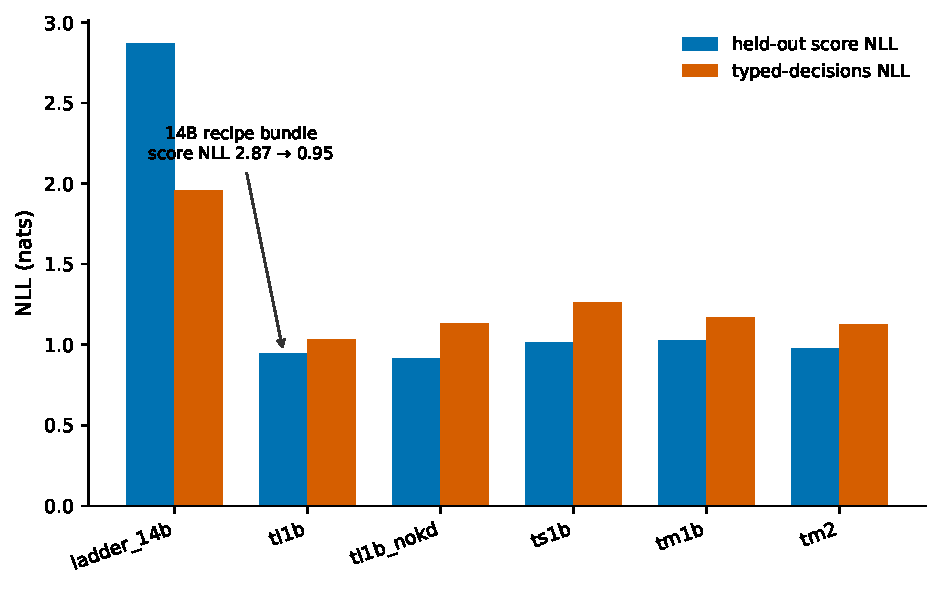
\includegraphics[width=\linewidth]{figures/fig_calibration.pdf}
  \caption{Held-out score NLL and typed-decisions NLL across the calibration-fix sequence (ladder\_14b $\rightarrow$ tl1b/tl1b\_nokd/ts1b/tm1b/tm2), showing the 2.87 $\rightarrow$ ~0.95 collapse fix.}
  \label{fig:calibration}
\end{figure}

\begin{figure}[t]
  \centering
  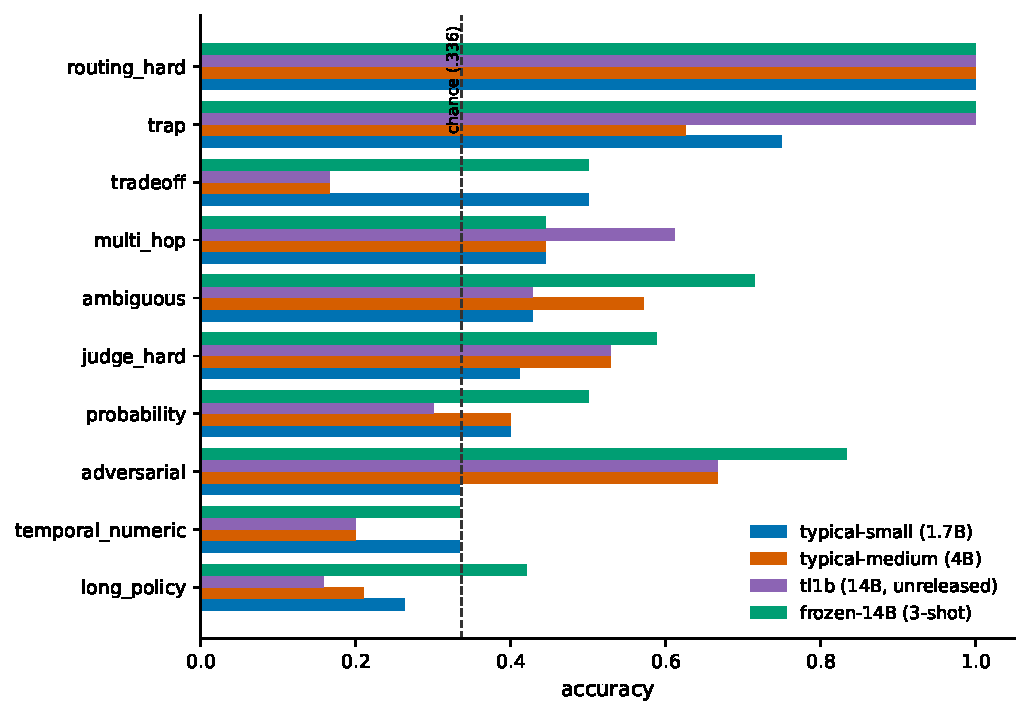
\includegraphics[width=\linewidth]{figures/fig_hard_families.pdf}
  \caption{Per-family JevBench-hard accuracy (10 families) for ladder\_14b, tl1b, and the frozen-14B 3-shot control, sorted by tl1b's value, with the chance line at .336. Note: ladder\_14b's temporal\_numeric/probability values here (.333/.50, re-derived from hard/results.jsonl) differ from REPORT.md 3ah's prose (.20/.40) -- the JSON artefact is used as the source of truth.}
  \label{fig:hard_families}
\end{figure}

\begin{figure}[t]
  \centering
  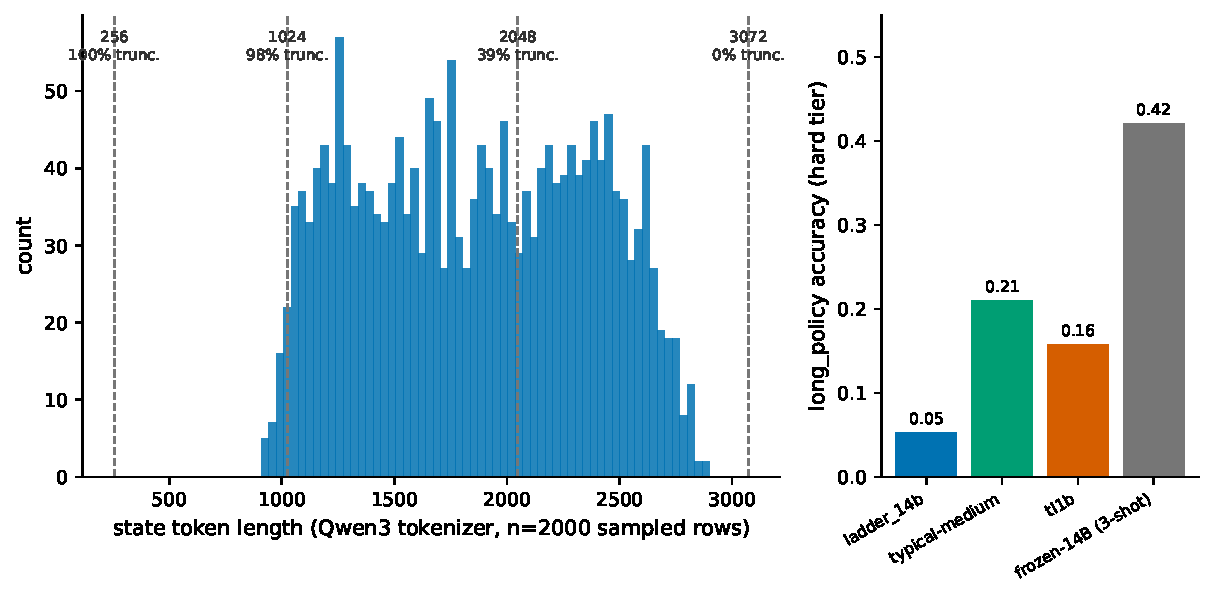
\includegraphics[width=\linewidth]{figures/fig_truncation.pdf}
  \caption{Left: histogram of data\_wf\_long state token lengths with truncation fractions at 256/1024/2048/3072 tokens. Right: long\_policy (hard-tier) accuracy across the long-state bug/fix sequence.}
  \label{fig:truncation}
\end{figure}

\begin{figure}[t]
  \centering
  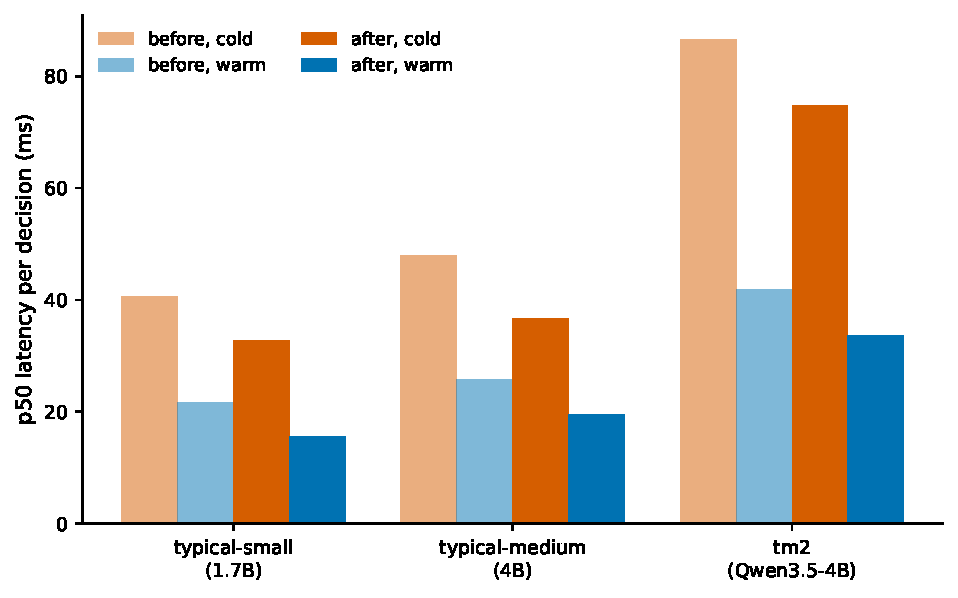
\includegraphics[width=\linewidth]{figures/fig_serving.pdf}
  \caption{Per-decision p50 latency before/after the zero-copy prefix fix, cold vs warm, for typical-small (1.7B), typical-medium (4B) and tm2 (Qwen3.5-4B), at K=2, state\_tokens=256.}
  \label{fig:serving}
\end{figure}
